\documentclass[conference]{IEEEtran}

\usepackage{amsmath}
\usepackage{booktabs}
\usepackage{graphicx}
\usepackage{url}
\usepackage{hyperref}

\title{Validating International Military Expenditure Data with Python}

\author{
\IEEEauthorblockN{Angel Morenu}
\IEEEauthorblockA{
Data Science Project\\
Email: angelhdbaez@gmail.com}
}

\begin{document}
\maketitle

\begin{abstract}
This paper presents a reproducible Python program for validating and analyzing
international military-expenditure data. The program checks required fields,
invalid values, duplicate country-year records, and aggregate classifications
before calculating descriptive statistics and observed world-spending growth.
In the executed run, 9,112 records were reviewed, 150 eligible country
observations were available for 2025, and world expenditure increased by
57.47\% from 1988 to 2025, equivalent to a 1.23\% compound annual growth
rate. The workflow also produces a logarithmic distribution chart while
handling zero expenditure values explicitly.
\end{abstract}

\begin{IEEEkeywords}
Python, data validation, military expenditure, descriptive statistics,
reproducible analysis, SIPRI
\end{IEEEkeywords}

\section{Objective}
The objective of this project is to build a transparent, repeatable workflow
for checking and analyzing international military-expenditure data. The
program loads a CSV or ZIP file, validates its structure, separates country
observations from aggregate rows, calculates 2025 country statistics, measures
world-level growth from observed values, and creates a distribution chart.

\section{Data and Method}
The input is the SIPRI Military Expenditure Database distributed through Our
World in Data. The series used in this analysis is expressed in constant 2024
U.S. dollars. The input loader accepts either the project CSV file or a ZIP
archive containing it.

The validation stage requires the columns \texttt{Entity}, \texttt{Year}, and
\texttt{Military expenditure}. Years and expenditures are converted to
numeric values. The program flags missing, non-finite, malformed, or negative
values and checks duplicate country-year groups. A three-letter country-code
pattern is used as a practical heuristic to separate country observations
from aggregate or unclassified records. Rows that fail the country
classification are excluded from country-level statistics rather than being
counted as countries.

For 2025, the program calculates the mean, median, and sample standard
deviation. It retains zero expenditure values in those statistics. Because
zero cannot be represented on a logarithmic axis, zero values are omitted only
from the distribution chart. World growth uses the first and last valid
observed \texttt{World} rows:
\begin{equation}
  \text{growth} =
  \frac{V_{\mathrm{last}}-V_{\mathrm{first}}}{V_{\mathrm{first}}}
  \times 100.
\end{equation}
The compound annual growth rate is calculated using the elapsed calendar
years between those endpoints.

\section{Program and Notebook}
Appendix A contains the Python programming example, executed outputs, and
visualization. An executable Jupyter notebook is also available as a
supplemental file.

\section{Executed Results}
Table~\ref{tab:results} reports the results from the executed notebook and
source CSV. The counts in this table are calculated by the program for this
run; they are not claims that apply to every future version of the source.

\begin{table}[!t]
\centering
\caption{Executed validation and analysis results.}
\label{tab:results}
\begin{tabular}{ll}
\toprule
\textbf{Measure} & \textbf{Result}\\
\midrule
Records reviewed & 9,112\\
Invalid years & 0\\
Invalid expenditures & 0\\
Duplicate country-years & 0\\
Aggregate/unclassified excluded & 771\\
Eligible 2025 countries & 150\\
Mean expenditure & \$18.266 billion\\
Median expenditure & \$1.285 billion\\
Sample standard deviation & \$82.608 billion\\
Positive chart observations & 147\\
World growth, 1988--2025 & 57.47\%\\
Compound annual growth rate & 1.23\%\\
\bottomrule
\end{tabular}
\end{table}

\subsection{Plain-language interpretation}
The program reviewed 9,112 records and found no invalid years, invalid
spending values, or duplicate country-year entries under its stated rules.
It excluded 771 aggregate or unclassified records from country analysis. For
2025, 150 eligible country observations averaged approximately \$18.266
billion, while the median observation was \$1.285 billion. The much larger
mean indicates that a small number of high-spending countries pull the
average upward.

The three zero-expenditure observations are Costa Rica, Iceland, and Panama.
They remain in the descriptive statistics but are omitted from the
logarithmic chart. The growth result uses 1988 as the first observed World
year and 2025 as the last; it therefore should not be presented as the
1998--2025 comparison used in a separate presentation.

\begin{figure}[!t]
\centering
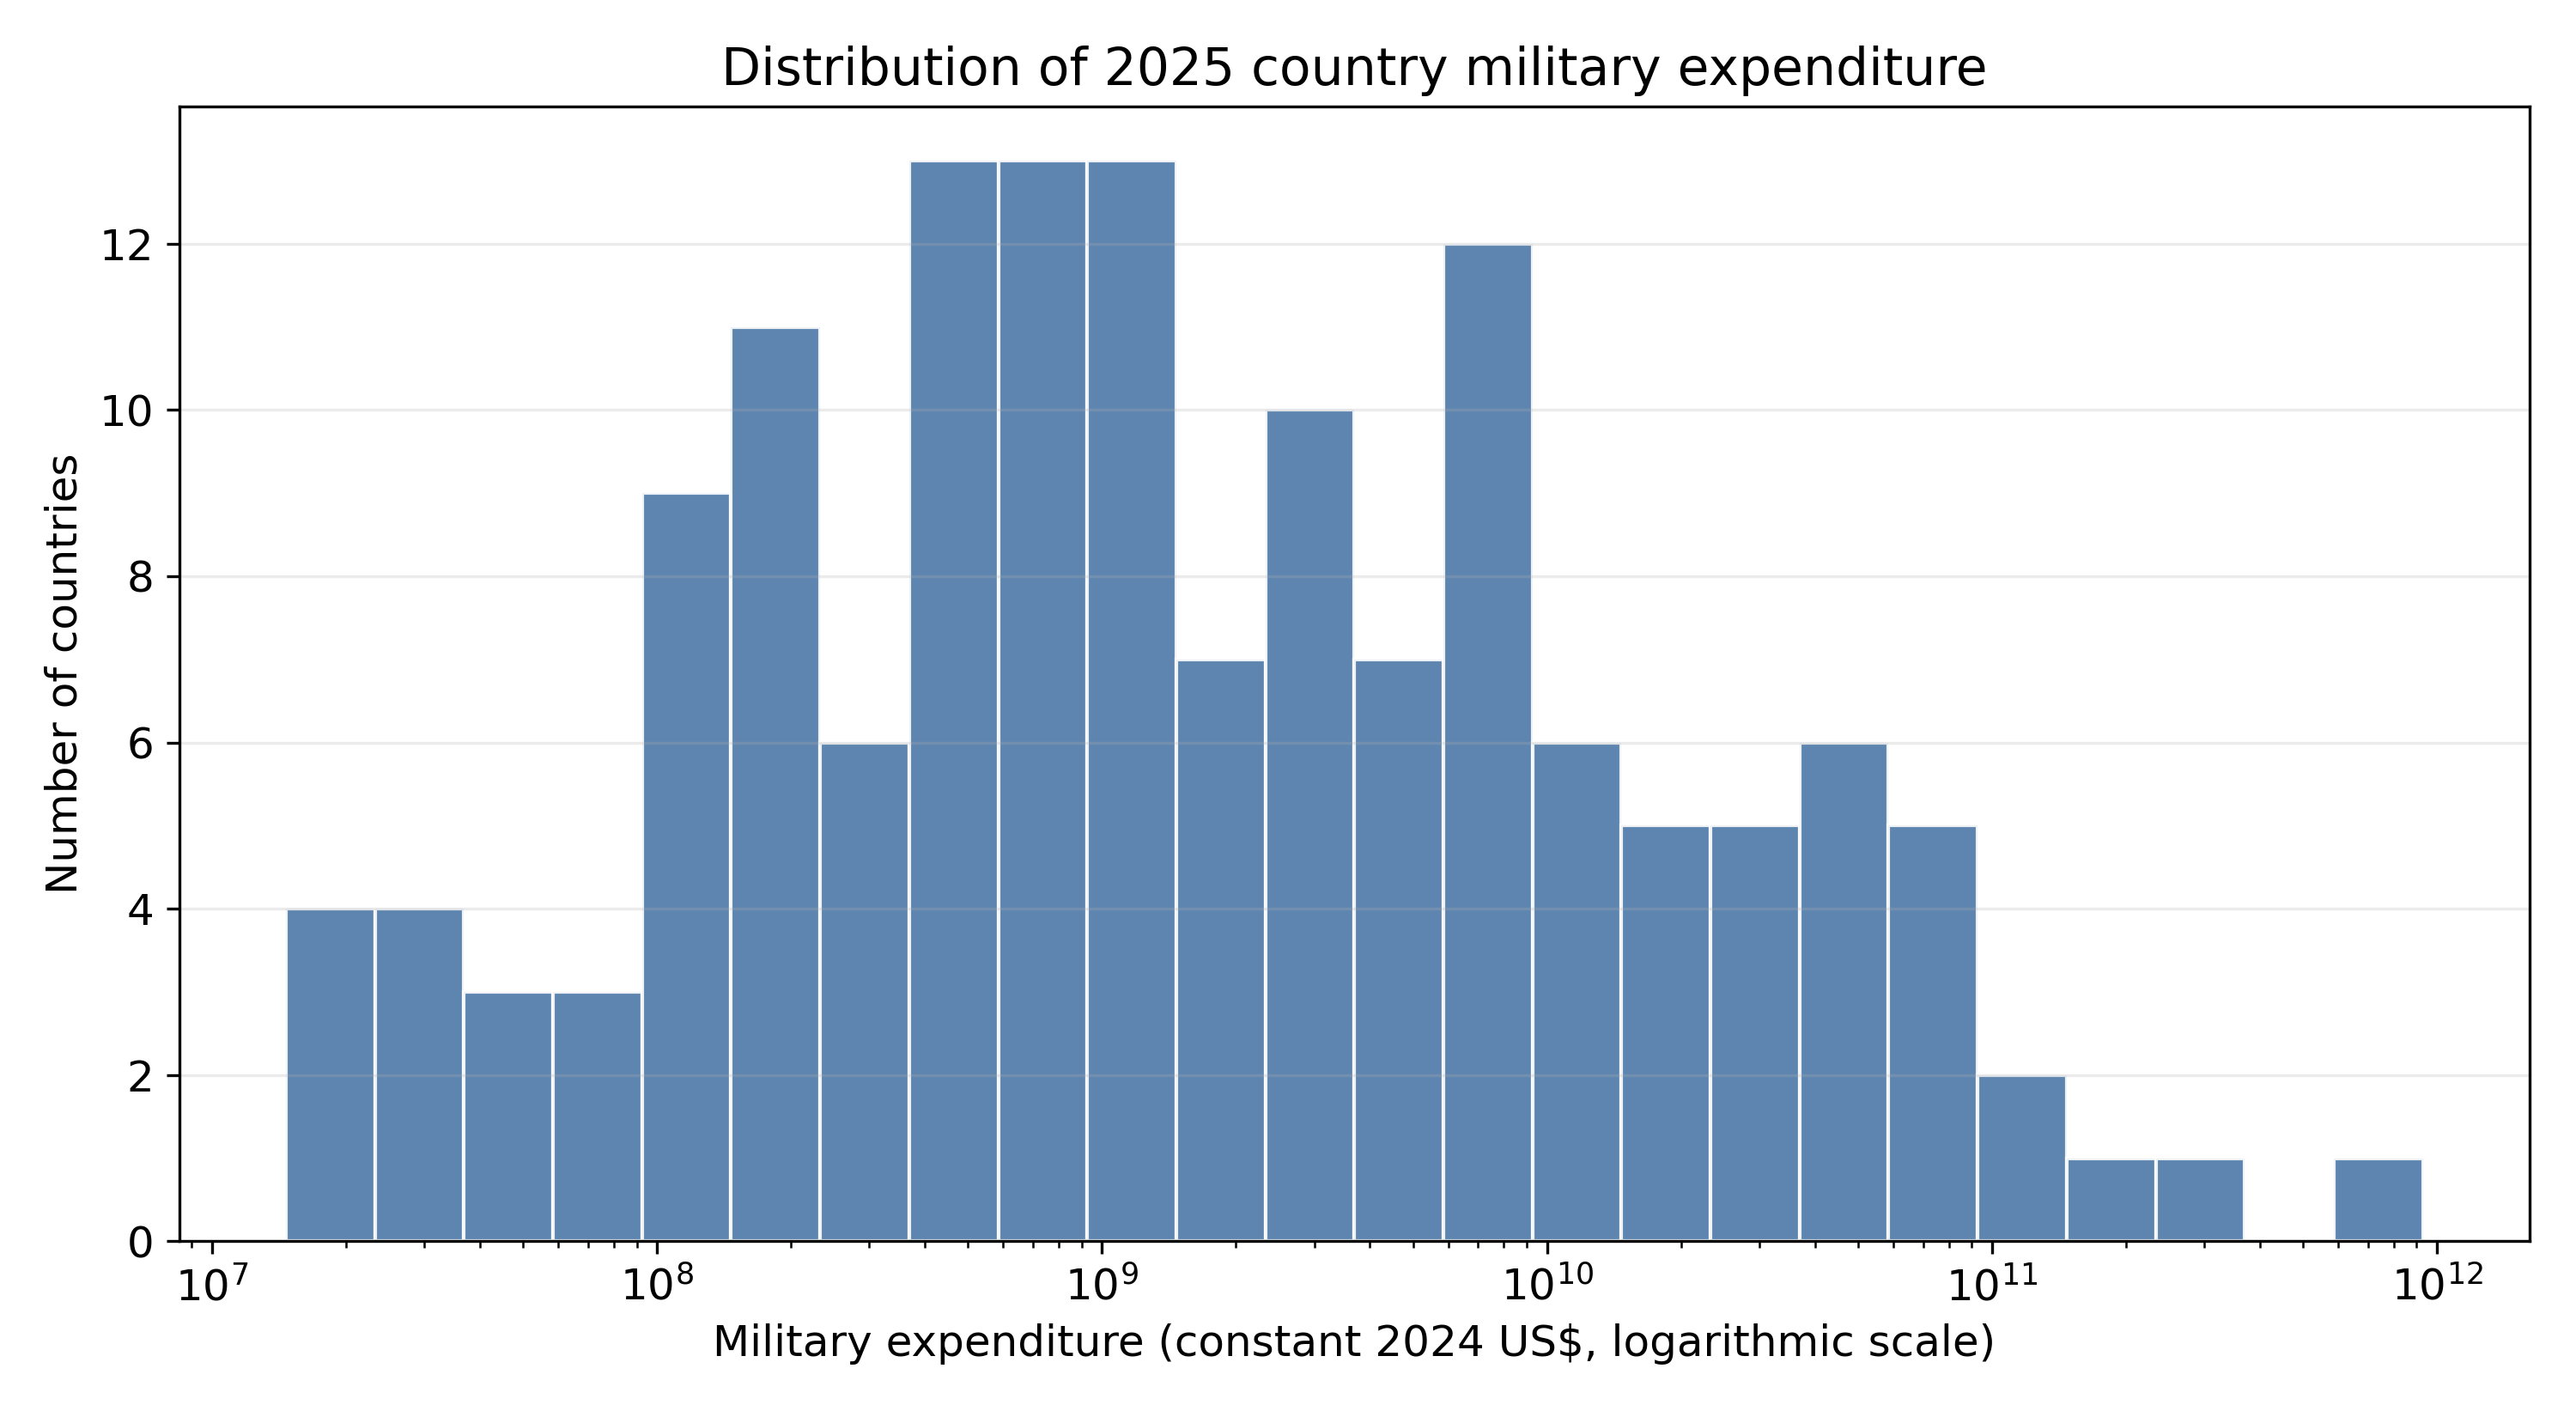
\includegraphics[width=\columnwidth]{outputs/military_expenditure_distribution_2025.png}
\caption{Distribution of eligible 2025 country expenditure. The logarithmic
chart displays 147 positive observations; three zero values are excluded
from the chart only.}
\label{fig:distribution}
\end{figure}

\begin{figure}[!t]
\centering
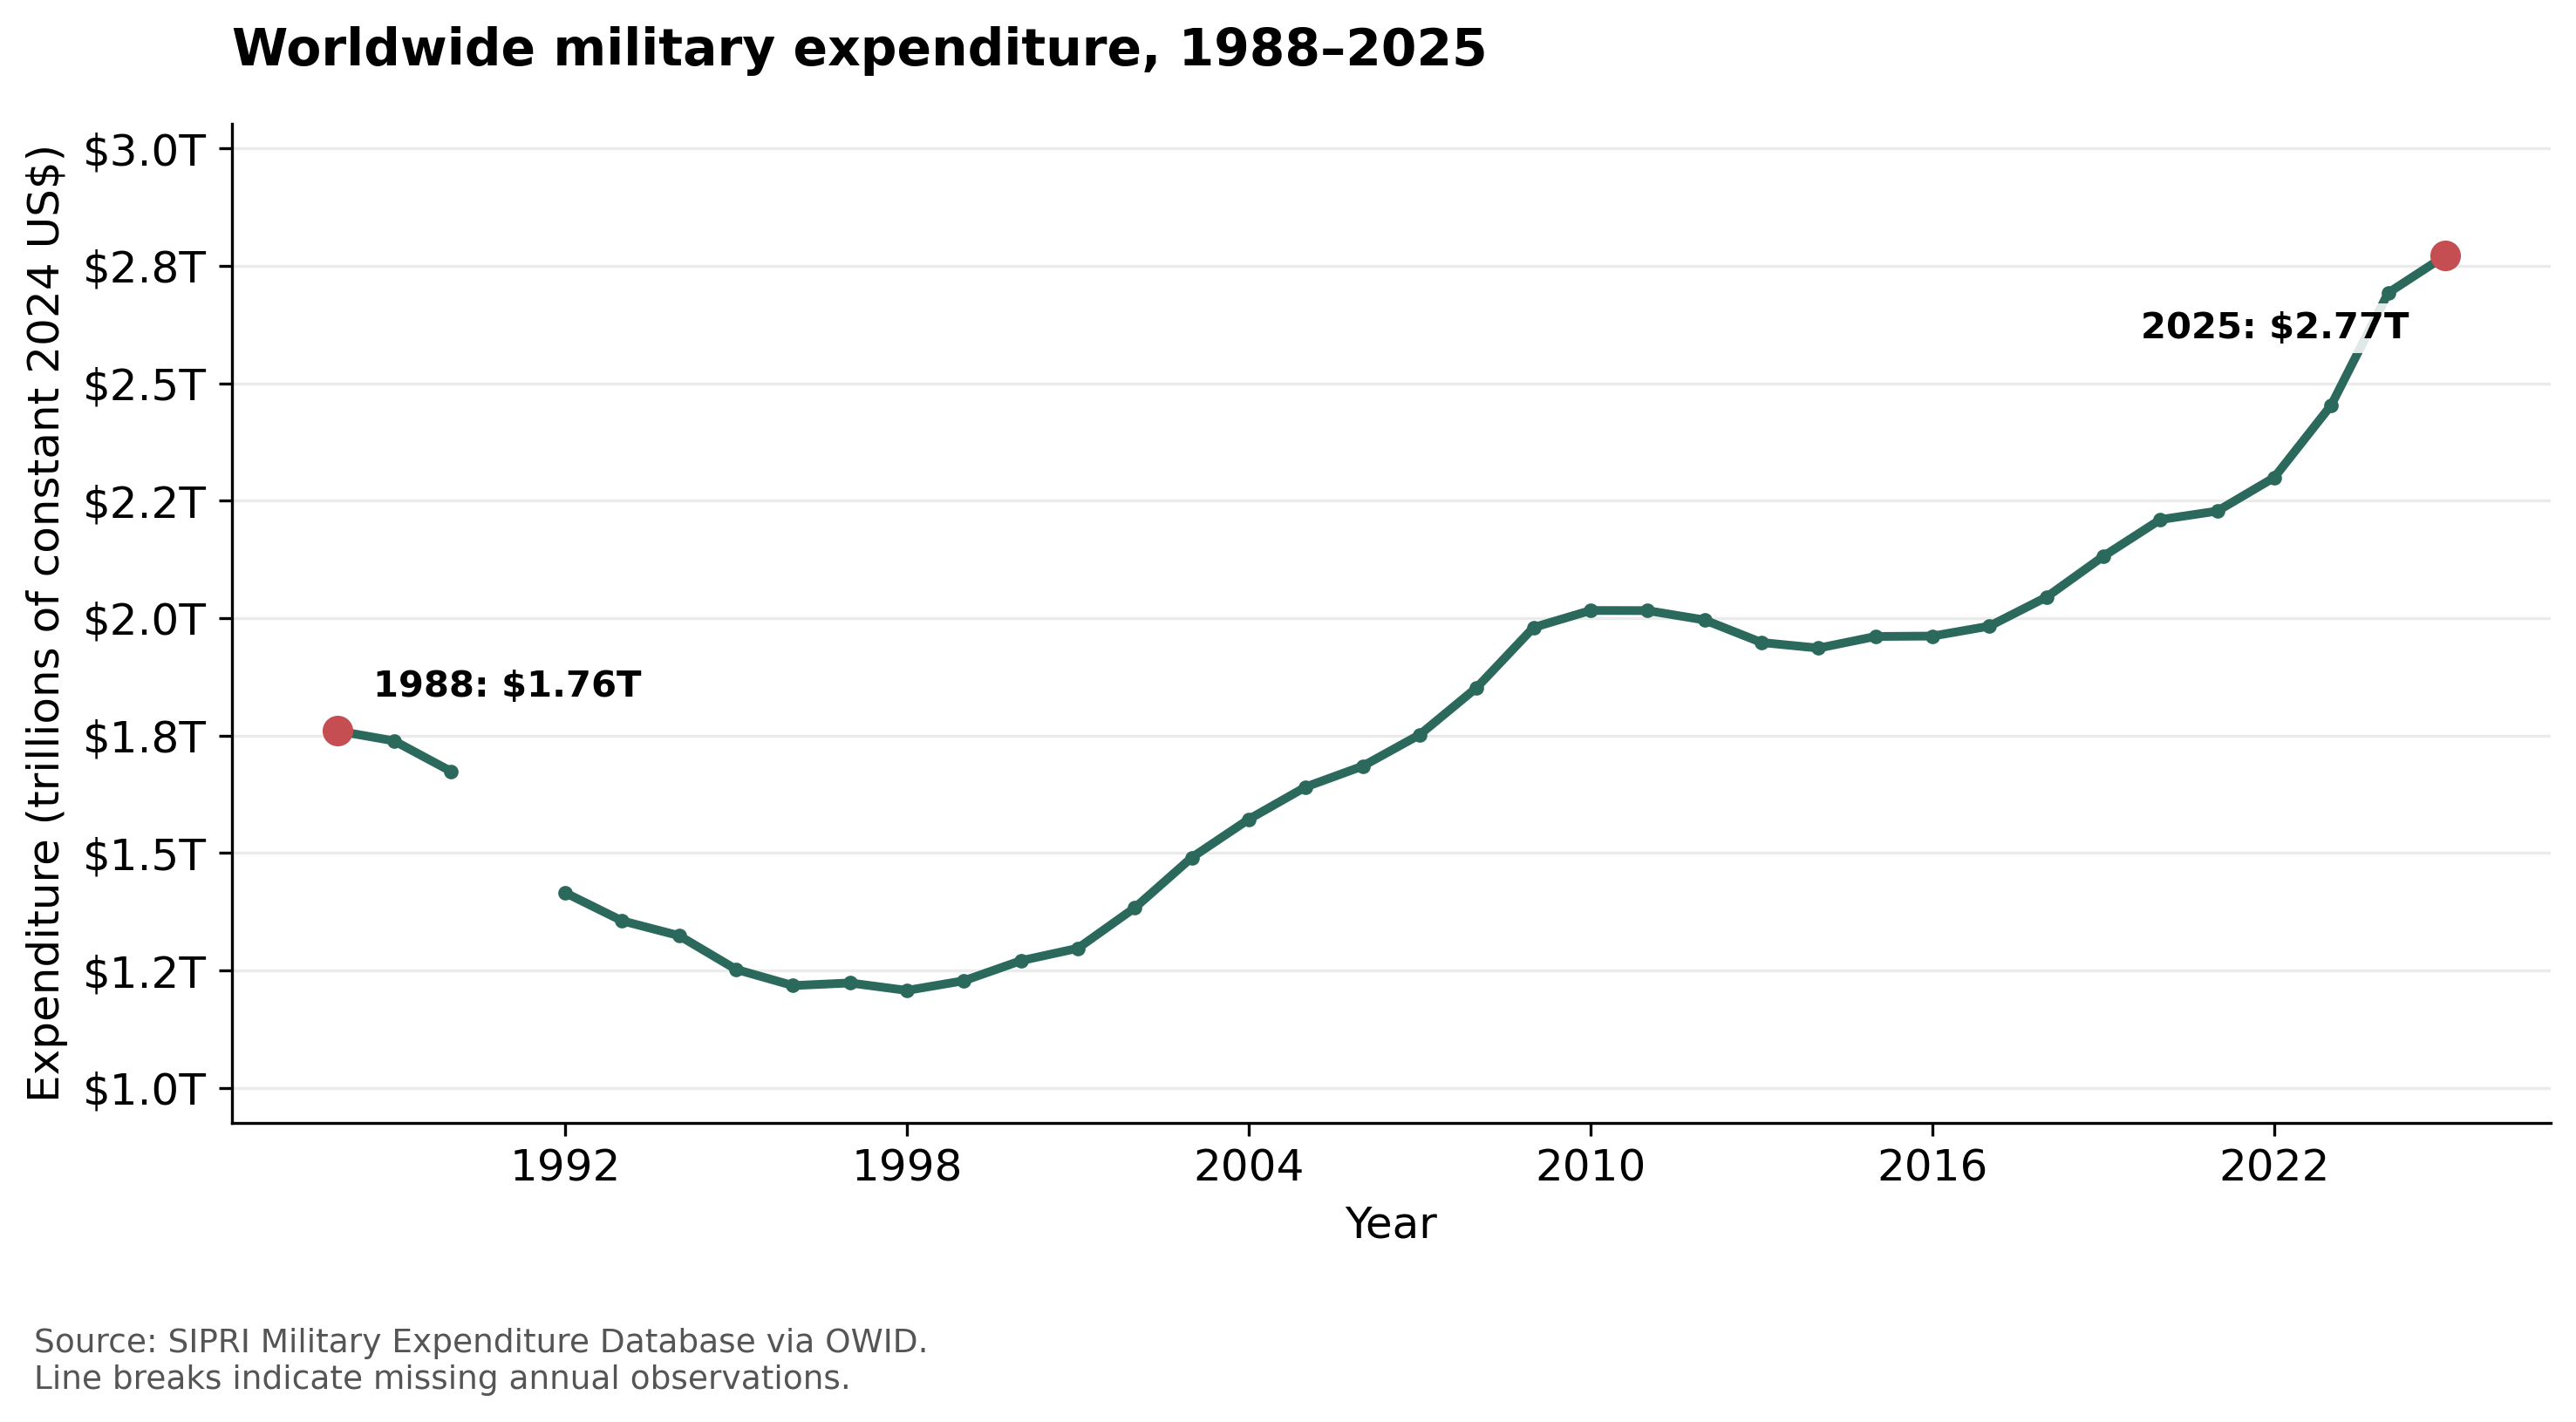
\includegraphics[width=\columnwidth]{outputs/world_military_expenditure_over_time.png}
\caption{Worldwide military expenditure increased from approximately
\$1.76 trillion in 1988 to \$2.77 trillion in 2025---a 57.47\% increase,
equivalent to compound annual growth of 1.23\%. These inflation-adjusted
figures show changes in spending over time. No valid worldwide expenditure
observation was available for 1991; the line breaks at that year, and no
interpolation was performed. The missing intermediate year does not prevent
calculating endpoint growth or CAGR for 1988--2025; those calculations use
the first and last valid values and elapsed calendar years.}
\label{fig:world-trend}
\end{figure}

\section{Limitations}
The checks validate selected structural properties, not the independent
accuracy of the source figures. The country classification uses a code-pattern
heuristic rather than an authoritative geopolitical classification. Missing
or nonstandard codes may exclude otherwise usable observations. Duplicate
country-year groups are excluded rather than reconciled, and endpoint CAGR
does not describe year-to-year volatility or establish causation. Source
metadata should also be reviewed for carried-forward or estimated values.

\section{Source and Authorship}
The source is the SIPRI Military Expenditure Database distributed through Our
World in Data. A project reference is SIPRI, ``Trends in World Military
Expenditure, 2025,'' April 2026, DOI:
\url{https://doi.org/10.55163/ZLHQ1057}.

The program and analysis were personally authored by Angel Morenu. AI
assistance was used for review and verification. The author the reviews the final code, executed
results, chart, and paper.

\section{Conclusion}
This project demonstrates how a small validation layer can make a data
analysis more reproducible and easier to interpret. The final workflow
combines structural checks, descriptive statistics, endpoint growth
calculations, and two complementary charts: one for differences across
countries and one for changes in worldwide spending over time.

\end{document}
